\documentclass{article}
\usepackage[hmargin=3cm, vmargin=3cm]{geometry}
\usepackage{graphicx}
\author{Ben Keller}
\title{Physics 785 Problem Set 1}
\begin{document}
\maketitle
\section{CGPS Spin Temperatures}
For this problem, the spin temperature $T_s$ was calculated using the same
equation as Strasser \& Taylor 2004:
$$ T_s = \frac{T_{boff}}{1-e^{-\tau}}$$
The error was in this was calculated using the partial derivatives:
$$ \delta T_s = \delta T_{boff} \frac{\partial T_s}{\partial T_{boff}} + \delta
	e^{-\tau} \frac{\partial T_s}{\partial e^{-\tau}}$$
$$ \delta T_s = \frac{\delta T_{boff}}{1-e^{-\tau}} + \frac{\delta
e^{-\tau}}{(e^{-\tau}-1)^2}$$

I also calculated a signal-to-noise value comparable to that used in Simon
Strasser's MSc thesis, and selected only spin temperatures where this value
was greater than 3 (ie, a $>3\sigma$ detection):
$$ SN = \frac{|T_{on}-T_{off}|}{\sqrt{\delta T_{on}^2 + \delta T_{off}^2}} $$
I also calculated the average spin temperature $\bar T_s$ of these three lines 
of sight for all channels that passed the previous criteria in all three lines 
of sight.  I also calculate an error for this average,
$$\delta \bar T_s = \sqrt{\delta T_{s1}^2+\delta T_{s2}^2+\delta
T_{s3}^2}/\sqrt{N}$$
This is shown in Figure 2, and
provides a similar picture as Figure 4.7 in the Strasser thesis:  since the 
LSR velocity is primarily a determined by projection of the galactic rotation
curve, this figure provides a view of the spin temperature at different depths 
in the galactic plane.
\begin{figure}
	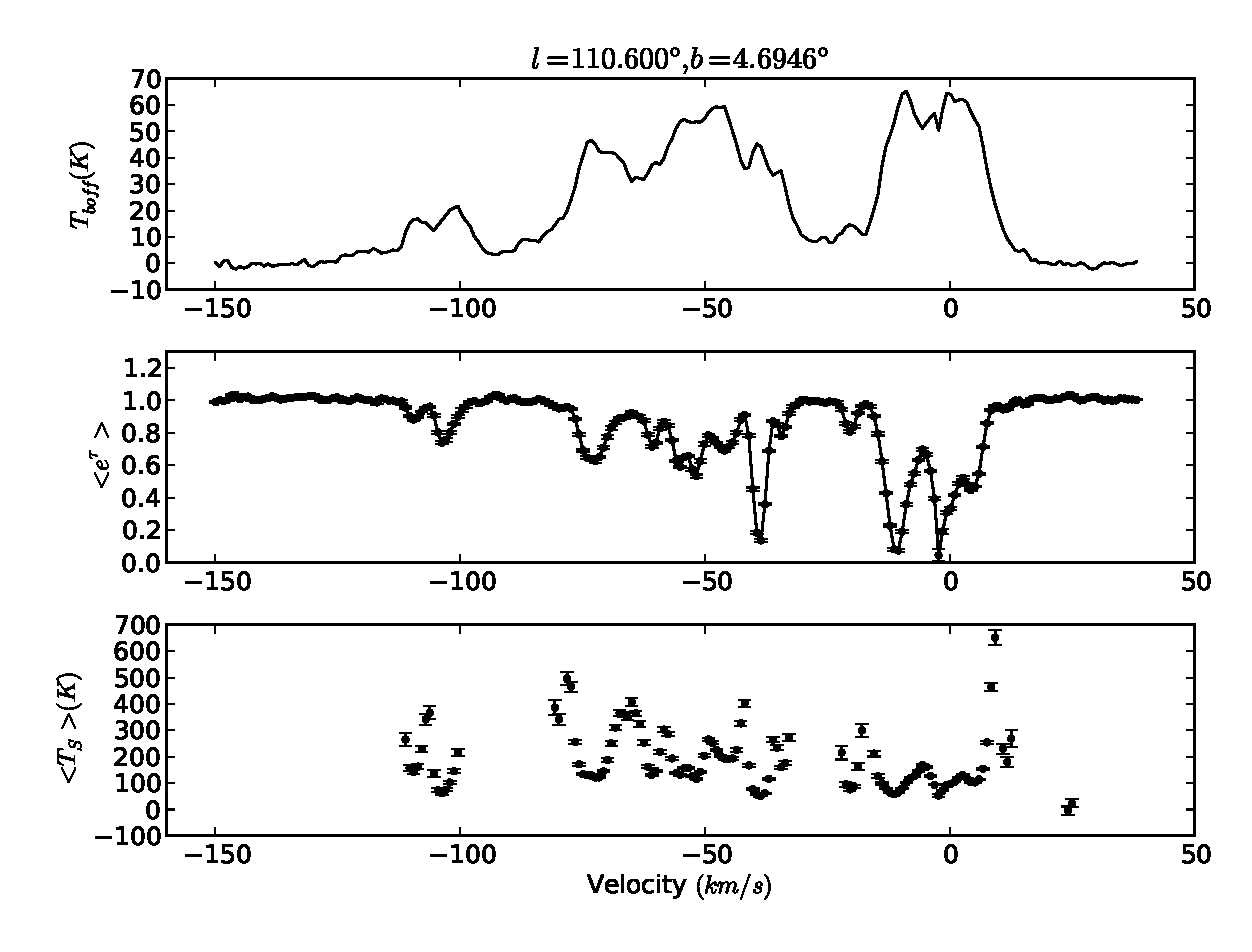
\includegraphics[scale=0.65]{110.600_4.6946.eps}
\end{figure}
\begin{figure}
	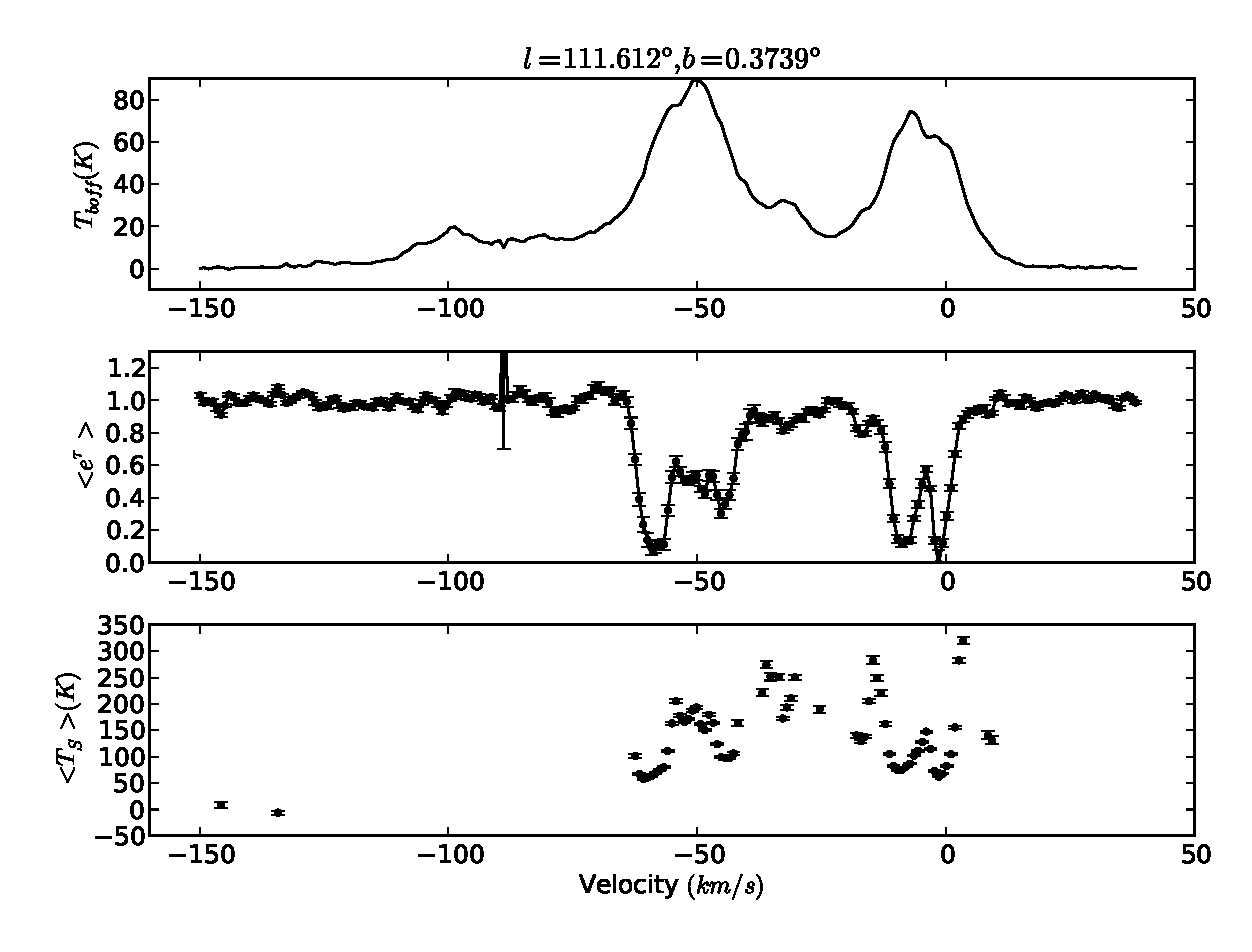
\includegraphics[scale=0.65]{111.612_0.3739.eps}
\end{figure}
\begin{figure}
	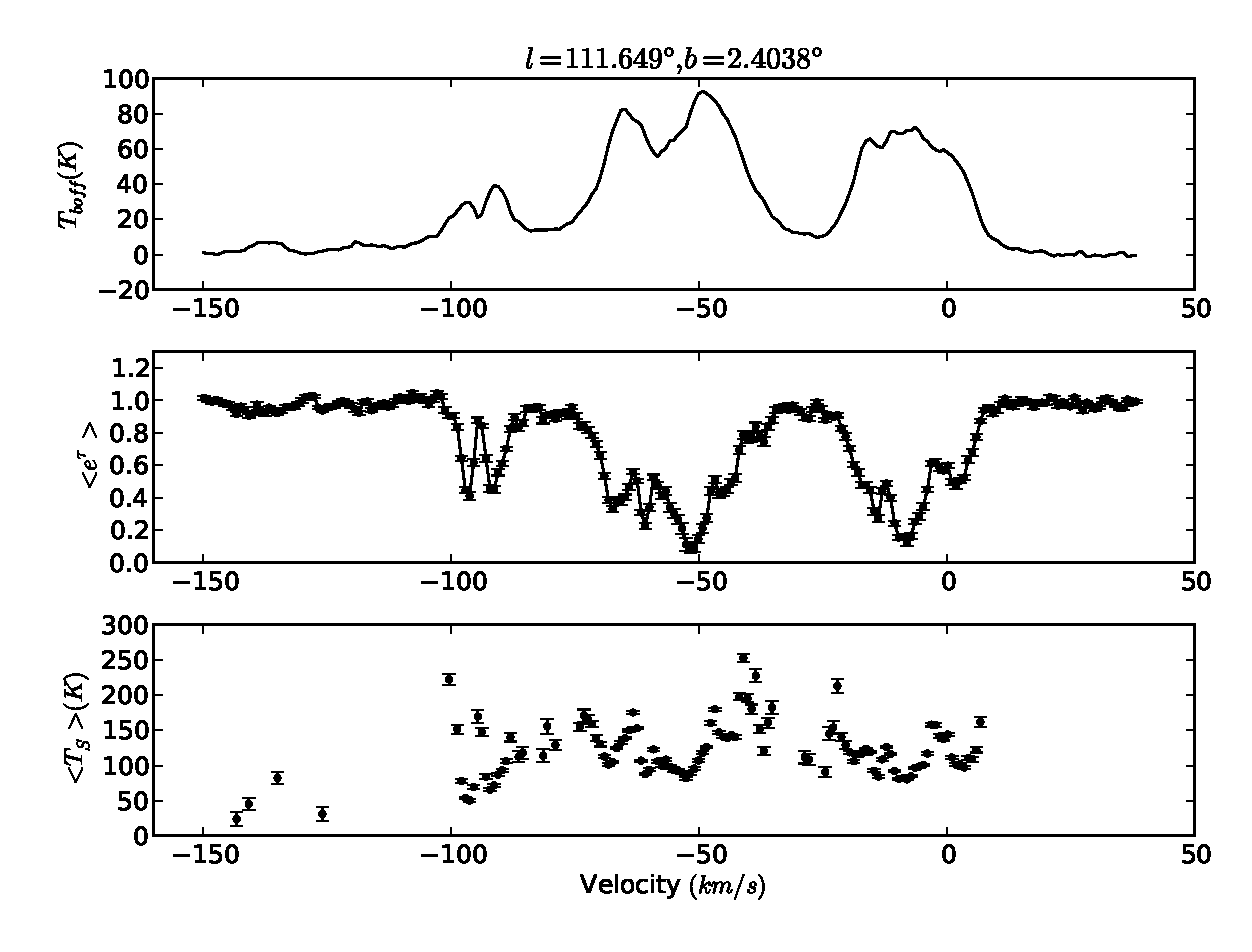
\includegraphics[scale=0.65]{111.649_2.4038.eps}
\caption{Off-source brightness temperature, exponential optical depth, and 
spin temperature for three lines of sight}
\end{figure}
\begin{figure}
	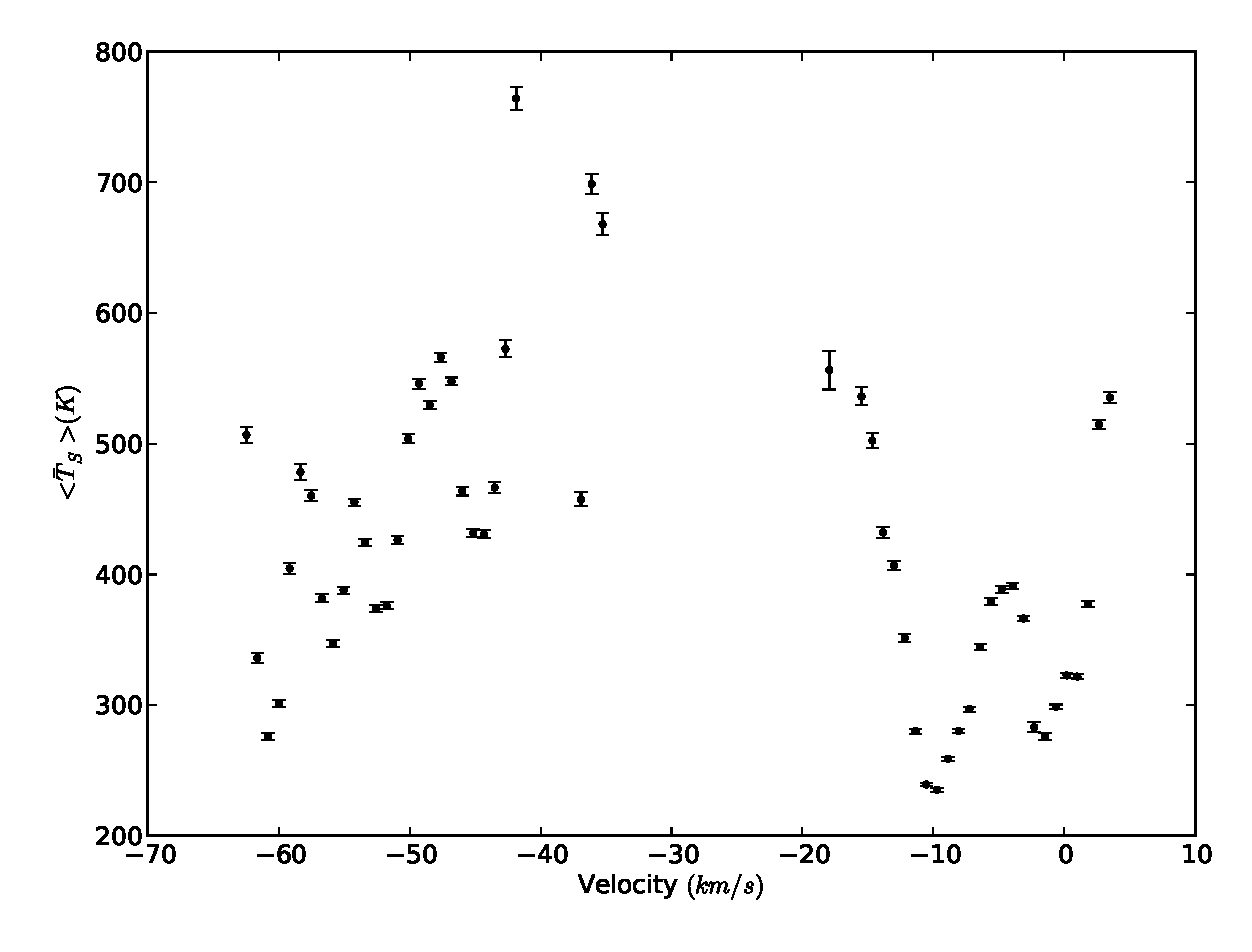
\includegraphics[scale=0.6]{meanTs.eps}
\caption{Mean spin temperature as a function of LSR velocity from 3 lines of
sight.}
\end{figure}
\pagebreak
\section{Cooling Function}
For the construction of a simple 3-component (Hydrogen, Carbon II, and Sulfur
II) cooling curve, used the following equations, derived from Dalgarno \& McCray
1972 for CII and from Penston 1970 for Hydrogen and SII.  The cooling component
I included for the two metals was \textit{Electron Impact Excitation} collisions
with HI.  The mechanism that HI cools in this function is through Lyman-$\alpha$
emission.  Each of these functions have had the density normalized out (but for
the diffuse ISM, the density can be expected to be $\approx 0.1 cm^{-3}$.  Also
omitted is the fractional ionization, which can become important in regions with
large cosmic ray or FUV flux.  In Figure 3, note the negative slope in
$\Lambda_{total}$ between  $\approx 200 - 4000 $K, indicative of a thermal
instability.  The abundances for CII and SII were obtained from Table 1 of 
Dalgarno \& McCray 1972.  The per-species cooling functions as a function of
temperatrue are shown below ($f_{CII}$ and $f_{SII}$ are the fractional
abundances of Carbon and Sulfur, and were set to $3.75*10^{-4}$ and
$1.4*10^{-5}$ respectively).
$$ \Lambda_{H} (T) = 10.2eV*3.23*10^{-10}T^{1/2}(1+17500/T)e^{-118000/T}$$
$$ \Lambda_{CII} (T) = f_{CII}*7.9*10^{-20}T^{-1/2}e^{-92/T}$$
$$ \Lambda_{SII} (T) = f_{SII}*8.44*10^{-18}T^{-1/2}e^{-21400/T}$$
\\
\\
\textit{Note: All calculations and plots were done using attached code}
\begin{figure}
	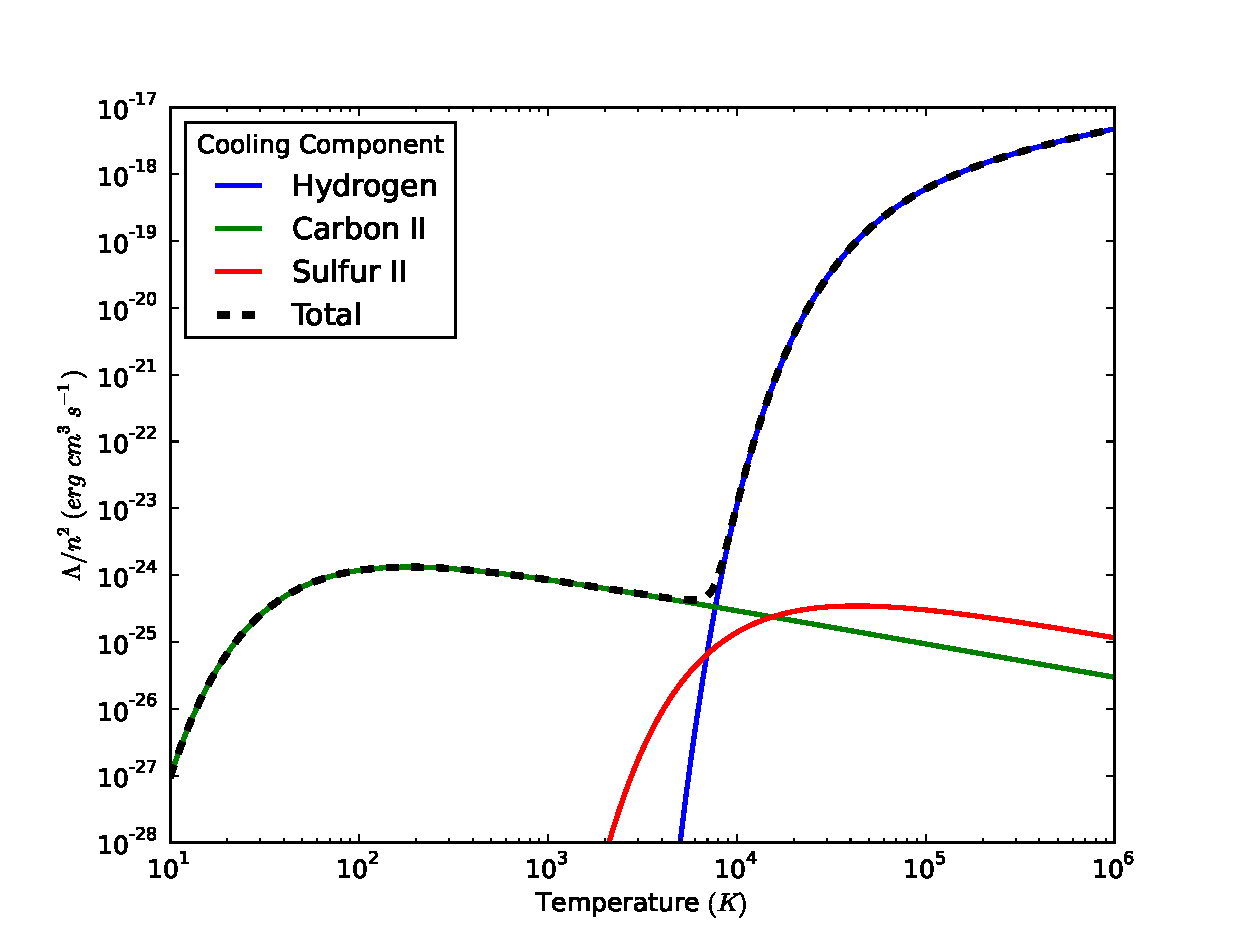
\includegraphics[scale=0.7]{cooling.eps}
\caption{Normalized cooling function for a diffuse ISM composed of Hydrogen,
Carbon, and Sulfur with typical abundances}
\end{figure}
\section*{References}
Penston, M.V., \textit{Cooling Mechanisms in the Interstellar Gas}, ApJ 162.
1970\\
Dalgarno, A. \& McCray, R.A., \textit{Heating and Ionization of HI Regions},
ARAA 10. 1972\\
Strasser, S.T., \textit{Properties of HI in the Galaxy}, University of Calgary
MSc Thesis. 2002\\
Strasser, S.T. \& Taylor, A.R. \textit{1420MHz Continuum Absorption toward
Extragalactic Sources in the Galactic Plane}, ApJ 603. 2004
\\
\\
\end{document}
